\documentclass[11pt,a4paper]{article}

\usepackage[utf8]{inputenc}
\usepackage[T1]{fontenc}
\usepackage{lmodern}
\usepackage[margin=1.1in]{geometry}
\usepackage{graphicx}
\usepackage{booktabs}
\usepackage{float}
\usepackage{xcolor}
\usepackage{hyperref}
\usepackage{enumitem}
\usepackage{amsmath}
\usepackage{mdframed}
\usepackage{subcaption}

\hypersetup{colorlinks=true, linkcolor=blue!60!black, urlcolor=blue!60!black}

\definecolor{accentblue}{RGB}{44,90,160}
\definecolor{lightblue}{RGB}{220,235,255}
\definecolor{lightgreen}{RGB}{220,245,220}
\definecolor{lightyellow}{RGB}{255,250,220}
\definecolor{lightred}{RGB}{255,230,230}
\definecolor{lightgray}{RGB}{245,245,245}

\newmdenv[backgroundcolor=lightblue,linecolor=accentblue,linewidth=1.5pt,
  innerleftmargin=12pt,innerrightmargin=12pt,
  innertopmargin=8pt,innerbottommargin=8pt]{keybox}
\newmdenv[backgroundcolor=lightgreen,linecolor=green!40!black,linewidth=1pt,
  innerleftmargin=12pt,innerrightmargin=12pt,
  innertopmargin=8pt,innerbottommargin=8pt]{findingbox}
\newmdenv[backgroundcolor=lightyellow,linecolor=orange!60!black,linewidth=1pt,
  innerleftmargin=12pt,innerrightmargin=12pt,
  innertopmargin=8pt,innerbottommargin=8pt]{notebox}
\newmdenv[backgroundcolor=lightred,linecolor=red!40!black,linewidth=1pt,
  innerleftmargin=12pt,innerrightmargin=12pt,
  innertopmargin=8pt,innerbottommargin=8pt]{warningbox}
\newmdenv[backgroundcolor=lightgray,linecolor=gray!50,linewidth=1pt,
  innerleftmargin=12pt,innerrightmargin=12pt,
  innertopmargin=8pt,innerbottommargin=8pt]{codebox}

\title{\textbf{The Partial Knowledge Paradox}\\[0.4em]
\large When the Agent Reads the Skill and Ignores It\\
2 Variants $\times$ 3 Runs on Spring PetClinic (Boot 4)\\[0.6em]
\normalsize Code Coverage Experiment v3}
\author{Dr.\ Mark Pollack}
\date{April 2026}

\begin{document}
\maketitle
\tableofcontents
\newpage

%% ============================================================
\section{What We Ran}

\subsection*{The question}

The v2 experiment showed that skills reduce search overhead by 25 percentage points
and prompt hardening is the single biggest quality driver. But v2 started from
\emph{zero} tests. What happens when the project already has tests --- and those
tests use older patterns?

The v3 experiment tests a specific hypothesis:
\textbf{when existing code contradicts skill guidance, the agent follows the code.}

This is the \emph{partial knowledge paradox}: the agent has access to correct
knowledge (via skills) but produces suboptimal output because it mimics
the patterns it finds in the existing codebase.

\subsection*{The task}

Write JUnit 5 tests for Spring PetClinic (Boot 4.0.1) to improve code coverage
from 65\% to at least 85\% line coverage. The project starts with 6 seed test files
that compile and pass but use \textbf{older patterns}:

\begin{itemize}
  \item \texttt{mockMvc.perform()} --- the established MockMvc API.
    Spring Framework 7 (which Boot 4 picks up) introduced \texttt{MockMvcTester},
    a fluent replacement with better AssertJ integration.
    Both APIs work; \texttt{MockMvcTester} is the recommended path forward.
  \item No \texttt{flush()}/\texttt{clear()} in \texttt{@DataJpaTest} classes ---
    a JPA testing best-practice gap. Without flushing and clearing the persistence
    context between writes and reads, assertions hit the Hibernate L1 cache
    rather than the database, masking potential bugs.
\end{itemize}

Skills explicitly teach the improved patterns.
The seed files demonstrate the older ones.

\subsection*{The setup}

\begin{itemize}
  \item \textbf{Model}: Claude Sonnet 4.6
  \item \textbf{Task}: improve coverage on spring-petclinic-partial (Boot 4.0.1)
  \item \textbf{Baseline}: 64.9\% line coverage (6 seed test files)
  \item \textbf{Coverage target}: $\geq$85\% via JaCoCo
  \item \textbf{Build}: \texttt{./mvnw clean test jacoco:report}
  \item \textbf{Runs}: 6 sessions total (N=3 per variant)
  \item \textbf{Skills}: \texttt{spring-mvc-testing}, \texttt{spring-jpa-testing},
    \texttt{spring-testing-fundamentals} (installed globally)
  \item \textbf{Tracking}: every tool call logged via \texttt{agent-journal}
\end{itemize}

\subsection*{The two variants}

This is not a 7-variant ladder. It is a controlled pair designed to isolate
one variable: prompt structure.

\begin{table}[H]
\centering
\renewcommand{\arraystretch}{1.2}
\begin{tabular}{@{}l p{9.5cm}@{}}
\toprule
\textbf{Variant} & \textbf{What the agent has} \\
\midrule
\texttt{simple}
  & Two-line prompt. ``Add JUnit tests to improve code coverage.''
    No process guidance. No stopping condition beyond a Done-When check. \\
\texttt{hardened-skills}
  & Seven-step structured prompt. Explicit stopping condition.
    Instruction to read existing tests first. Guidance on slice selection,
    version-aware patterns, and what \emph{not} to test. \\
\bottomrule
\end{tabular}
\caption{Two variants tested. Both have access to the same skills.
Both start from the same 6 seed files with older patterns.}
\end{table}

\subsection*{What we measured}

Three tiers of automated judges:

\begin{itemize}
  \item \textbf{T0 (BuildSuccess)}: \texttt{./mvnw clean test jacoco:report} exits 0.
    Fail = reject immediately.
  \item \textbf{T1 (CoverageImprovement)}: JaCoCo line coverage $\geq$85\%
    and improvement from baseline. Normalized 0--1.
  \item \textbf{T2 (TestQuality)}: LLM judge scoring 6 criteria with \texttt{grep}-enforced
    checks. Range 0.0--1.0 per criterion.
\end{itemize}

Tool calls were classified into 9 semantic states for Markov chain analysis
(EXPLORE, SHELL, READ\_KB, READ\_SKILL, JAR\_INSPECT, WRITE, BUILD, VERIFY, FIX).
Journal analysis answered 6 behavioral questions about skill consumption, read order,
redundant reads, and cost distribution.

%% ============================================================
\section{The Smoking Gun}
\label{sec:smoking-gun}

Every run tells the same story. Here is run n1/hardened-skills, tool calls 5--28:

\begin{codebox}
\begin{verbatim}
 [ 5] Skill(spring-mvc-testing)        <- reads the skill
 [ 6] Read(mvc-rest-testing-patterns.md) <- reads the reference doc
     ... reads existing tests, production code ...
 [28] Write(PetControllerTests.java)    <- writes with mockMvc.perform()
\end{verbatim}
\end{codebox}

The skill teaches \texttt{MockMvcTester}. The agent reads it.
The agent then reads the existing \texttt{OwnerControllerTests.java},
which uses \texttt{mockMvc.perform()}.
When it writes its own controller test, it uses \texttt{mockMvc.perform()}.

This pattern repeats in \textbf{all 6 runs}, both variants.
The T2 judge catches it:

\begin{center}
\renewcommand{\arraystretch}{1.3}
\begin{tabular}{@{}lcc@{}}
\toprule
\textbf{T2 Criterion} & \textbf{Score} & \textbf{Passed?} \\
\midrule
test\_slice\_selection          & 1.00 & Yes \\
assertion\_quality              & 0.80 & Yes \\
error\_and\_edge\_case\_coverage & 0.80 & Yes \\
domain\_specific\_test\_patterns & \textbf{0.30} & \textbf{No} \\
coverage\_target\_selection      & 0.80 & Yes \\
version\_aware\_patterns         & \textbf{0.30} & \textbf{No} \\
\midrule
\textbf{Average (T2)}          & \textbf{0.667} & --- \\
\bottomrule
\end{tabular}
\end{center}

Criteria 4 and 6 fail because of the two seed-file defects:
\begin{itemize}
  \item \textbf{version\_aware\_patterns = 0.30}: Zero \texttt{MockMvcTester} occurrences,
    17--18 \texttt{mockMvc.perform()} calls across 5 files. The judge's \texttt{grep}
    enforcement: Boot 4+ projects using \texttt{mockMvc.perform()} score 0.30 max.
  \item \textbf{domain\_specific\_test\_patterns = 0.30}: Zero \texttt{flush()}/\texttt{clear()}
    calls in \texttt{@DataJpaTest}. The judge's \texttt{grep}: \texttt{save()} then
    \texttt{findById()} without \texttt{flush()+clear()} = Hibernate L1 cache false positive.
\end{itemize}

\begin{warningbox}
\textbf{T2 = 0.667 across all 6 runs.} Both variants. Every session.
The quality ceiling is set by the seed files, not by the prompt or the skills.
The 4 criteria the agent passes (slice selection, assertion quality, error coverage,
target selection) reflect the model's strong baseline on a known domain.
The 2 it fails reflect the exemplar's pull.
\end{warningbox}

%% ============================================================
\section{Two-Axis Results}
\label{sec:results}

\begin{table}[H]
\centering
\renewcommand{\arraystretch}{1.3}
\begin{tabular}{@{}lrrrrrr@{}}
\toprule
\textbf{Variant} & \textbf{N} & \textbf{Mean cost} & \textbf{$\pm$} &
  \textbf{Mean turns} & \textbf{T2 quality} & \textbf{Final cov.} \\
\midrule
\texttt{simple}            & 3 & \$3.60 & 0.54 & 47.0 & 0.667 & 95.2\% \\
\texttt{hardened-skills}   & 3 & \$3.46 & 0.72 & 46.7 & 0.667 & 92.9\% \\
\bottomrule
\end{tabular}
\caption{Summary results. Cost, turns, and coverage vary across runs;
T2 quality is invariant.}
\end{table}

\begin{table}[H]
\centering
\renewcommand{\arraystretch}{1.3}
\begin{tabular}{@{}llrrrrrrr@{}}
\toprule
\textbf{Run} & \textbf{Variant} & \textbf{Cost} & \textbf{Turns} &
  \textbf{Duration} & \textbf{Baseline} & \textbf{Final} & \textbf{T1} & \textbf{T2} \\
\midrule
n1 & simple            & \$4.07 & 42 & 20.3 min & 64.9\% & 95.3\% & 0.608 & 0.667 \\
n1 & hardened-skills   & \$3.99 & 52 & 16.9 min & 64.9\% & 94.6\% & 0.595 & 0.667 \\
n2 & simple            & \$3.72 & 52 & 18.0 min & 64.9\% & 94.6\% & 0.595 & 0.667 \\
n2 & hardened-skills   & \$2.62 & 37 & 12.5 min & 64.9\% & 89.2\% & 0.486 & 0.667 \\
n3 & simple            & \$3.00 & 47 & 13.0 min & 64.9\% & 95.6\% & 0.615 & 0.667 \\
n3 & hardened-skills   & \$3.77 & 51 & 16.4 min & 64.9\% & 94.9\% & 0.601 & 0.667 \\
\bottomrule
\end{tabular}
\caption{Per-run breakdown. All 6 runs pass T0 (build success). T2 = 0.667 is invariant.
T1 varies because coverage ranges from 89.2\% to 95.6\%.}
\end{table}

\begin{notebox}
\textbf{The n2/hardened-skills outlier}: 37 turns, \$2.62, 89.2\% coverage.
This is the cheapest run in the dataset --- but also the lowest coverage.
The agent wrote fewer tests and stopped earlier. It still passed T0 (build success)
and cleared the 85\% minimum, but produced less thorough coverage than the other 5 runs.
\end{notebox}

%% ============================================================
\section{Four Key Findings}

\begin{findingbox}
\textbf{Finding 1: The exemplar controls quality, not the skill.}

All 6 runs: T2 = 0.667. Both variants. The agent reads the skill
(spring-mvc-testing teaches \texttt{MockMvcTester}), reads the reference document,
then writes \texttt{mockMvc.perform()} because that's what the seed files demonstrate.

The skill fires in every run. It is consumed (the agent reads it).
It is ignored in practice. The existing code is the stronger signal.

\emph{What the agent sees beats what the agent is told.}
\end{findingbox}

\begin{findingbox}
\textbf{Finding 2: The behavioral fingerprint differs even when quality converges.}

Both variants produce T2 = 0.667. But they get there differently.

\begin{center}
\begin{tabular}{@{}lcc@{}}
\toprule
\textbf{Metric} & \textbf{simple} & \textbf{hardened-skills} \\
\midrule
Orientation phase          & 72\% of calls  & 65\% of calls \\
First file read            & \texttt{PetClinicApplication.java} & \texttt{pom.xml} \\
Read order                 & production code first & existing tests first \\
Redundant reads per run    & 16.7 & 4.3 \\
Avg tool calls             & 84   & 61 \\
Expected steps (Markov)    & 260  & 164 \\
\bottomrule
\end{tabular}
\end{center}

\texttt{simple} reads every production file, then re-reads them when it needs
to write tests. \texttt{hardened-skills} reads existing tests first (as instructed),
infers what's needed, and avoids re-reading. The 37\% reduction in expected steps
is real efficiency --- it just doesn't manifest as quality because the quality
ceiling is set by the exemplar.
\end{findingbox}

\begin{findingbox}
\textbf{Finding 3: Redundant reads are the concrete inefficiency.}

\texttt{simple}: 16.7 redundant file reads per run (files read $\geq$2 times).
\texttt{hardened-skills}: 4.3 redundant reads per run. A 4$\times$ difference.

The \texttt{simple} agent reads production source files, writes tests, then re-reads
the same files to write more tests. It does not retain file content across
turns. The \texttt{hardened-skills} agent reads production files once
because the prompt directs it to survey coverage gaps first, then write.

Each redundant read costs tokens (cache read tokens, but still billed)
and adds a tool-call round trip.
\end{findingbox}

\begin{findingbox}
\textbf{Finding 4: PetClinic coverage converges regardless.}

All 6 runs reach 89--96\% line coverage from a 64.9\% baseline.
This confirms the v2 finding: Spring PetClinic is the model floor ---
the model knows this domain and produces adequate coverage with any prompt.

The v3 contribution is showing that coverage convergence coexists with
quality divergence that the exemplar controls. The model gets the lines
covered but uses the older API because the seed files demonstrate that pattern.
\end{findingbox}

%% ============================================================
\section{The Behavioral Signature}
\label{sec:behavioral}

\subsection*{Two different paths to the same destination}

The Markov chain analysis reveals fundamentally different navigation patterns
despite identical outcomes.

\begin{figure}[H]
\centering
\begin{minipage}[t]{0.48\textwidth}
  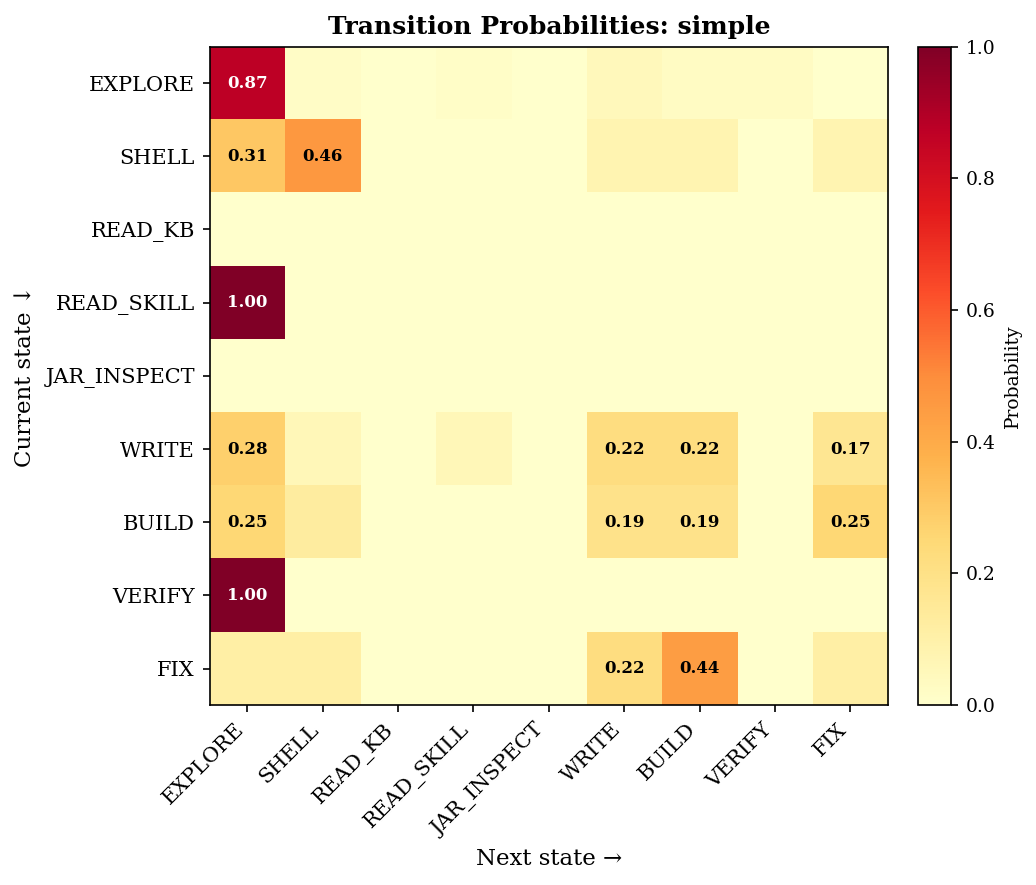
\includegraphics[width=\textwidth]{../figures/heatmap-simple.png}
  \caption*{\textbf{simple}: EXPLORE self-loop at 87\%. The agent
            reads, re-reads, reads again. Orientation-heavy.}
\end{minipage}\hfill
\begin{minipage}[t]{0.48\textwidth}
  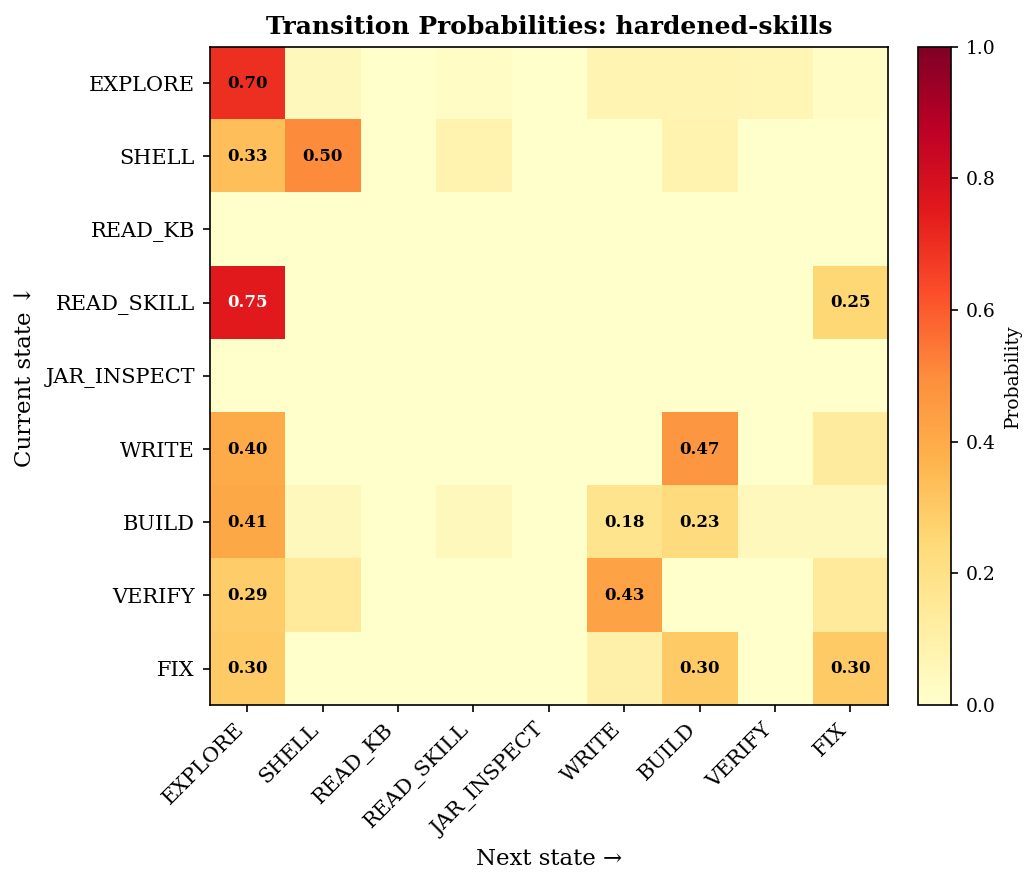
\includegraphics[width=\textwidth]{../figures/heatmap-hardened-skills.png}
  \caption*{\textbf{hardened-skills}: EXPLORE self-loop at 70\%.
            More transitions to WRITE and BUILD.}
\end{minipage}
\caption{Transition probability heatmaps. The EXPLORE self-loop dominance
         in \texttt{simple} means the agent is stuck reading files rather than
         writing tests. \texttt{hardened-skills} exits the reading phase sooner.}
\end{figure}

\begin{figure}[H]
\centering
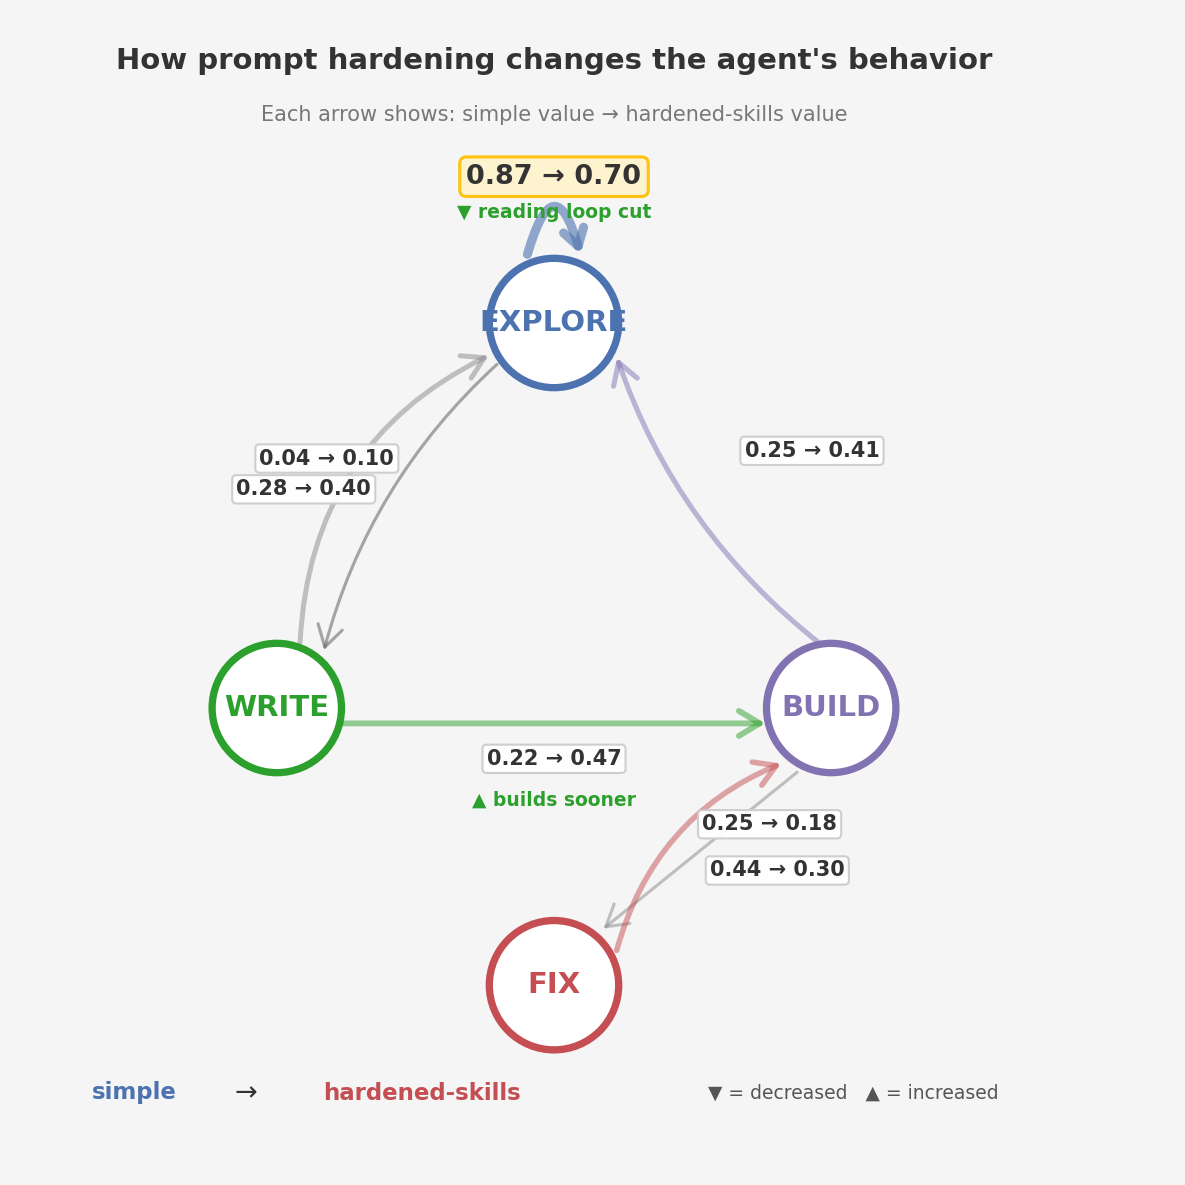
\includegraphics[width=0.75\textwidth]{../figures/state-diagram-combined.png}
\caption{Combined state diagram showing both variants on a single graph.
         Each arrow shows: \texttt{simple} value $\to$ \texttt{hardened-skills} value.
         Two changes stand out: the EXPLORE self-loop drops from 0.87 to 0.70
         (the agent spends less time re-reading files), and the WRITE$\to$BUILD
         transition more than doubles (0.22 $\to$ 0.47) --- the agent writes a test
         and immediately builds it instead of returning to read more files.}
\end{figure}

\subsection*{The Markov numbers}

\begin{center}
\renewcommand{\arraystretch}{1.3}
\begin{tabular}{@{}lrrrrr@{}}
\toprule
\textbf{Variant} & \textbf{P(success)} & \textbf{Exp. steps} &
  \textbf{FIX\_LOOP \%} & \textbf{SEARCH \%} & \textbf{JAR\_INSPECT \%} \\
\midrule
\texttt{simple}            & 1.000 & 260.3 & 11.0\% & 6.2\% & 0.0\% \\
\texttt{hardened-skills}   & 1.000 & 164.0 & 20.1\% & 7.3\% & 0.0\% \\
\bottomrule
\end{tabular}
\end{center}

Both variants have P(success) = 1.0 and JAR\_INSPECT = 0\%. The zero
JAR inspection is expected: PetClinic's dependencies are standard Spring Boot
starters, and Boot 4 import paths are in the model's training data.

The 37\% reduction in expected steps (260 $\to$ 164) comes from the
\texttt{hardened-skills} prompt breaking the EXPLORE self-loop:
the agent reads fewer files, re-reads less, and transitions to WRITE sooner.

\begin{notebox}
\textbf{Loop amplification}: The EXPLORE state has 189$\times$ amplification in
\texttt{simple} vs.\ 93$\times$ in \texttt{hardened-skills}. This means an agent
starting in EXPLORE is expected to visit that state 189 times before exiting in the
simple variant --- a direct measure of the ``reading treadmill'' the unstructured
prompt creates.
\end{notebox}

\subsection*{FIX\_LOOP: higher in hardened-skills}

Counterintuitively, \texttt{hardened-skills} has a higher FIX\_LOOP percentage
(20.1\% vs.\ 11.0\%). This is because the hardened prompt includes explicit
instructions to verify compilation after each batch of writes
(\emph{``Run \texttt{./mvnw compile} --- do NOT proceed if compilation fails.
Fix it first.''}). The agent follows this instruction: it builds more often,
catches errors earlier, and fixes them. The \texttt{simple} agent writes more
files before attempting a build, so its FIX/BUILD ratio is lower but its
failures are larger.

Both variants average 1.0 fix cycles per run --- PetClinic is easy enough that
neither variant spirals.

\begin{figure}[H]
\centering
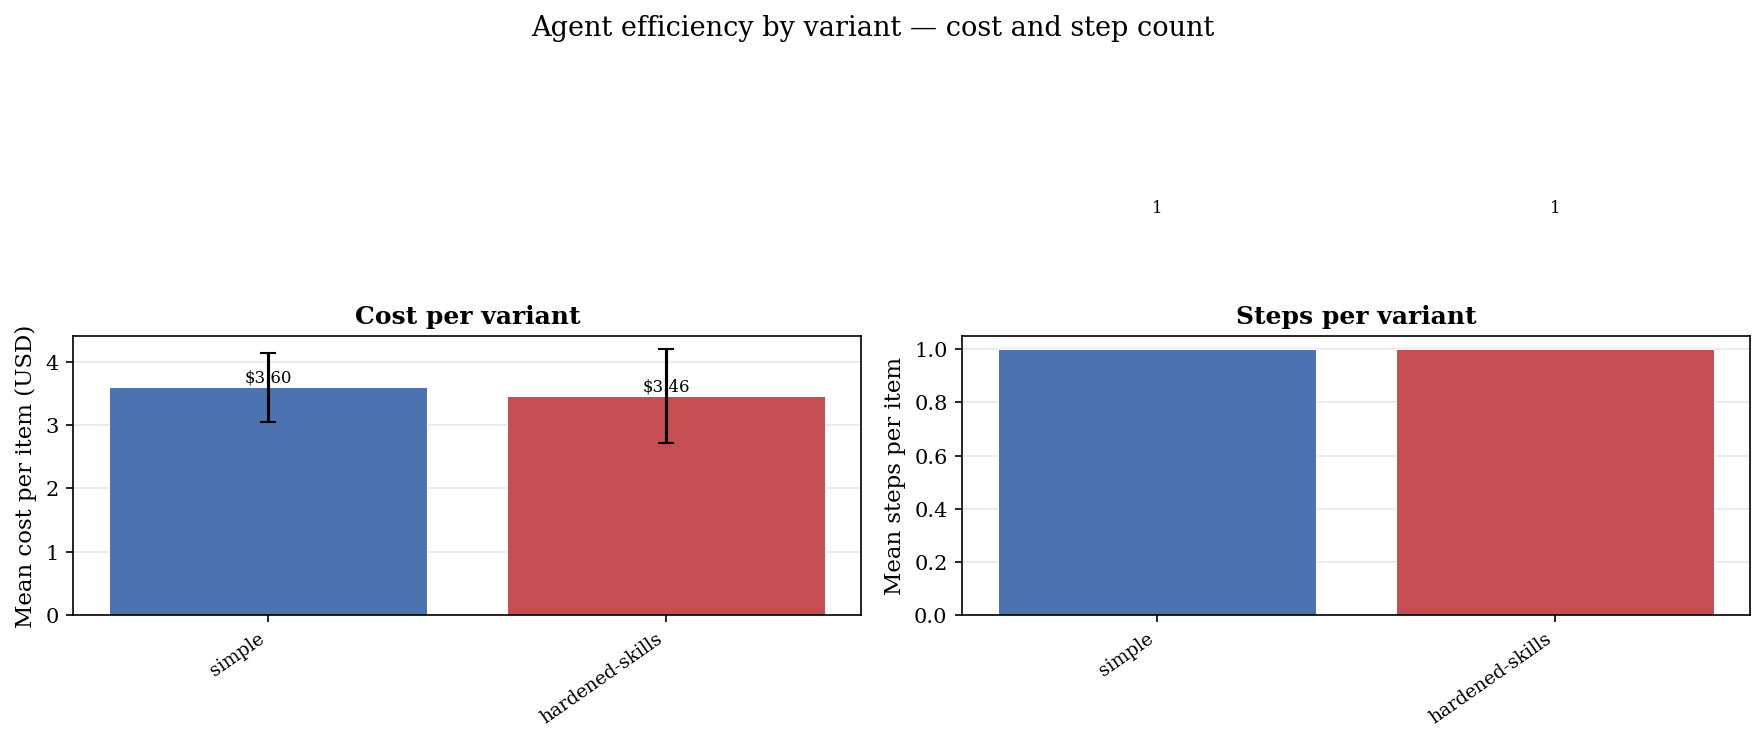
\includegraphics[width=0.85\textwidth]{../figures/cost-steps-comparison.png}
\caption{Cost (left) and step count (right) by variant. The difference
         is modest in absolute terms because PetClinic is a simple task ---
         the behavioral divergence is larger than the cost divergence.}
\end{figure}

%% ============================================================
\section{The Exemplar Effect: v2 vs.\ v3}
\label{sec:exemplar-effect}

The v2 experiment started from \textbf{zero tests}. No seed files.
Nothing for the agent to mimic.

The v3 experiment starts from \textbf{6 seed test files} using older patterns.
Skills are identical. The model is identical.

\begin{table}[H]
\centering
\renewcommand{\arraystretch}{1.3}
\begin{tabular}{@{}lccl@{}}
\toprule
& \textbf{v2 (zero tests)} & \textbf{v3 (seed files)} & \textbf{What changed} \\
\midrule
Coverage (simple)    & 92--94\% & 89--96\% & Converges either way \\
T2/T3 quality        & 0.783--0.878 & 0.667  & Exemplar patterns cap quality \\
version\_aware       & 0.70--1.00   & \textbf{0.30}   & Seed files use \texttt{perform()} \\
domain\_specific     & 0.70--0.90   & \textbf{0.30}   & Seeds lack flush/clear \\
JAR\_INSPECT         & 1.7--17.7\%  & \textbf{0.0\%}  & Boot 4 imports are known \\
\bottomrule
\end{tabular}
\caption{v2 vs.\ v3 comparison. The seed files pull down the two criteria that
  depend on adopting improved APIs. Quality on the other 4 criteria is comparable.}
\end{table}

\begin{warningbox}
\textbf{The paradox}: In v2, the agent sometimes discovered the correct patterns on its
own (T3 scores up to 0.878). In v3, with explicit skill guidance \emph{and} a structured
prompt, the agent scores 0.667 --- because the seed files are a stronger signal than
the skills. Providing knowledge does not help when the codebase contradicts it.
\end{warningbox}

This is the central finding of v3. The v2 experiment showed that knowledge injection
(skills, KB) improves efficiency. v3 shows the boundary condition:
\textbf{knowledge injection fails when existing code provides a contradictory exemplar.}

%% ============================================================
\section{What This Experiment Cannot Show}
\label{sec:limits}

\begin{warningbox}
\textbf{Same petclinic ceiling as v2.}

PetClinic is still the model floor. Coverage converges to 89--96\%
regardless of variant. The coverage axis is not a discriminator.

The T2 quality axis \emph{is} a discriminator --- but only because the seed files
create a measurable defect. On a project with correct seed files,
both variants would score identically on T2 as well.
\end{warningbox}

\textbf{What v3 does prove}:
\begin{itemize}
  \item The exemplar effect is real and measurable: 6/6 runs,
    consistent across variants and sessions.
  \item Behavioral fingerprints differ even when outcomes converge ---
    observable via Markov analysis and journal inspection.
  \item Redundant reads are a concrete, quantifiable efficiency tax
    (16.7 vs.\ 4.3 per run).
  \item The model reads skills, reads references, and still follows
    the code. This is not a routing failure --- it is a precedence failure.
\end{itemize}

\textbf{What v3 does not prove}:
\begin{itemize}
  \item Whether fixing the seed files would raise T2 above 0.667.
    (The v2 data suggests yes: without seed files, T3 reached 0.878.)
  \item Whether the exemplar effect holds on codebases the model
    does not know. (On novel domains, the model may rely more on skills
    because it has less prior knowledge to fall back on.)
  \item Whether stronger prompt intervention (``ignore existing patterns,
    use MockMvcTester'') would override the exemplar signal.
    This is a v4 variant hypothesis.
\end{itemize}

%% ============================================================
\section{Implications for Practice}
\label{sec:implications}

\begin{keybox}
\textbf{Three takeaways for anyone running coding agents:}

\begin{enumerate}[leftmargin=1.5em,itemsep=4pt]
  \item \textbf{Fix the exemplar before optimizing the prompt.}
    The agent will mimic what it sees. If the existing tests use the older API,
    the agent will use the older API. No amount of skill guidance overrides
    the codebase. Update the seed files first.

  \item \textbf{Behavioral differences are invisible in pass/fail metrics.}
    Both variants pass every judge. Both produce $\sim$90--95\% coverage.
    The 4$\times$ difference in redundant reads and the 37\% difference
    in expected steps are only visible in the tool-call trace.
    If you only measure outcomes, you miss the efficiency story.

  \item \textbf{Knowledge injection is an efficiency tool, not a quality tool,
    on known domains.}
    Skills reduce EXPLORE amplification from 189$\times$ to 93$\times$.
    They do not improve quality when the model already knows the domain.
    The quality lever is the exemplar.
\end{enumerate}
\end{keybox}

%% ============================================================
\section{What Comes Next}
\label{sec:next}

Two follow-up experiments are planned:

\subsection*{v4: Fix the exemplar}

Same task, same codebase. Replace the 6 seed test files with versions that use
\texttt{MockMvcTester} and include \texttt{flush()}/\texttt{clear()}.
Re-run both variants.

\textbf{Prediction}: T2 rises to $\geq$0.85 (matching v2's hardened quality)
because the exemplar and the skill now agree. The skill becomes reinforcement
rather than a contradicted suggestion.

This is the cheapest possible experiment: 6 files changed, 6 runs, same infrastructure.

\subsection*{Fineract: novel domain}

The v2 report's planned follow-up. Apache Fineract (banking, Gradle, Spring Boot 3.2.2).
Novel domain the model does not know well.

On a novel domain, the model cannot fall back on training data.
Skills should have a \emph{quality} effect, not just an efficiency effect.
The seed-file exemplar effect may be weaker because the model
has less certainty about what patterns to follow.

%% ============================================================
\section{The Short Summary}

\begin{keybox}
\textbf{What the v3 experiment shows:}

\begin{enumerate}[leftmargin=1.5em,itemsep=4pt]
  \item \textbf{The agent reads the skill and ignores it.}
    6/6 runs: skill consumed, reference read, old pattern written.
    The existing code is a stronger signal than structured knowledge.

  \item \textbf{T2 = 0.667 is a hard ceiling set by the seed files.}
    4 criteria pass (slice, assertion, error, target). 2 fail
    (domain patterns, version awareness). Both failures trace directly
    to defects in the seed test files.

  \item \textbf{The behavioral fingerprint diverges even when quality converges.}
    \texttt{simple}: 260 expected steps, 16.7 redundant reads, production-first.
    \texttt{hardened-skills}: 164 expected steps, 4.3 redundant reads, test-first.
    A 37\% efficiency difference invisible in pass/fail metrics.

  \item \textbf{Fix the code, not the prompt.}
    Prompt hardening and skills improve how the agent navigates.
    They do not override what the agent imitates.
    The highest-leverage intervention is updating the exemplar.
\end{enumerate}

\vspace{6pt}
\textbf{The v3 punchline}: Knowledge injection works --- but the codebase
is the agent's primary teacher. If the codebase demonstrates older patterns,
no skill can override them.
\end{keybox}

\end{document}
